\subsection{Messreihe zur Bestimmung der Zeitkonstanten im RC-Kreis}
In der ersten Messreihe die Zeitkonstante gemessen.
Die aufgebaute Schaltung wird durch Abbildung \ref{fig:Aufbau1} beschrieben.
Es ist ein Kondensator mit der Kapazität C und ein Widerstand mit dem Ohm'schen Widerstand R zu sehen.
Diese sind an einen Spannungsgenerator und ein Oszilloskop angeschlossen.
Am Spannungsgenerator wird eine Rechteckspannung $U_{0}(t)$ eingestellt.
Auf dem Oszilloskop sind die Auflade- und Entladevorgänge im Spannungsverlauf des Kondensator $U_{C}(t)$ zu sehen.
Mit der Cursorfunktion des Oszilloskops werden 30 Werte für $U_{C}(t)$ abgelesen.

\begin{figure}[h!]
  \centering
  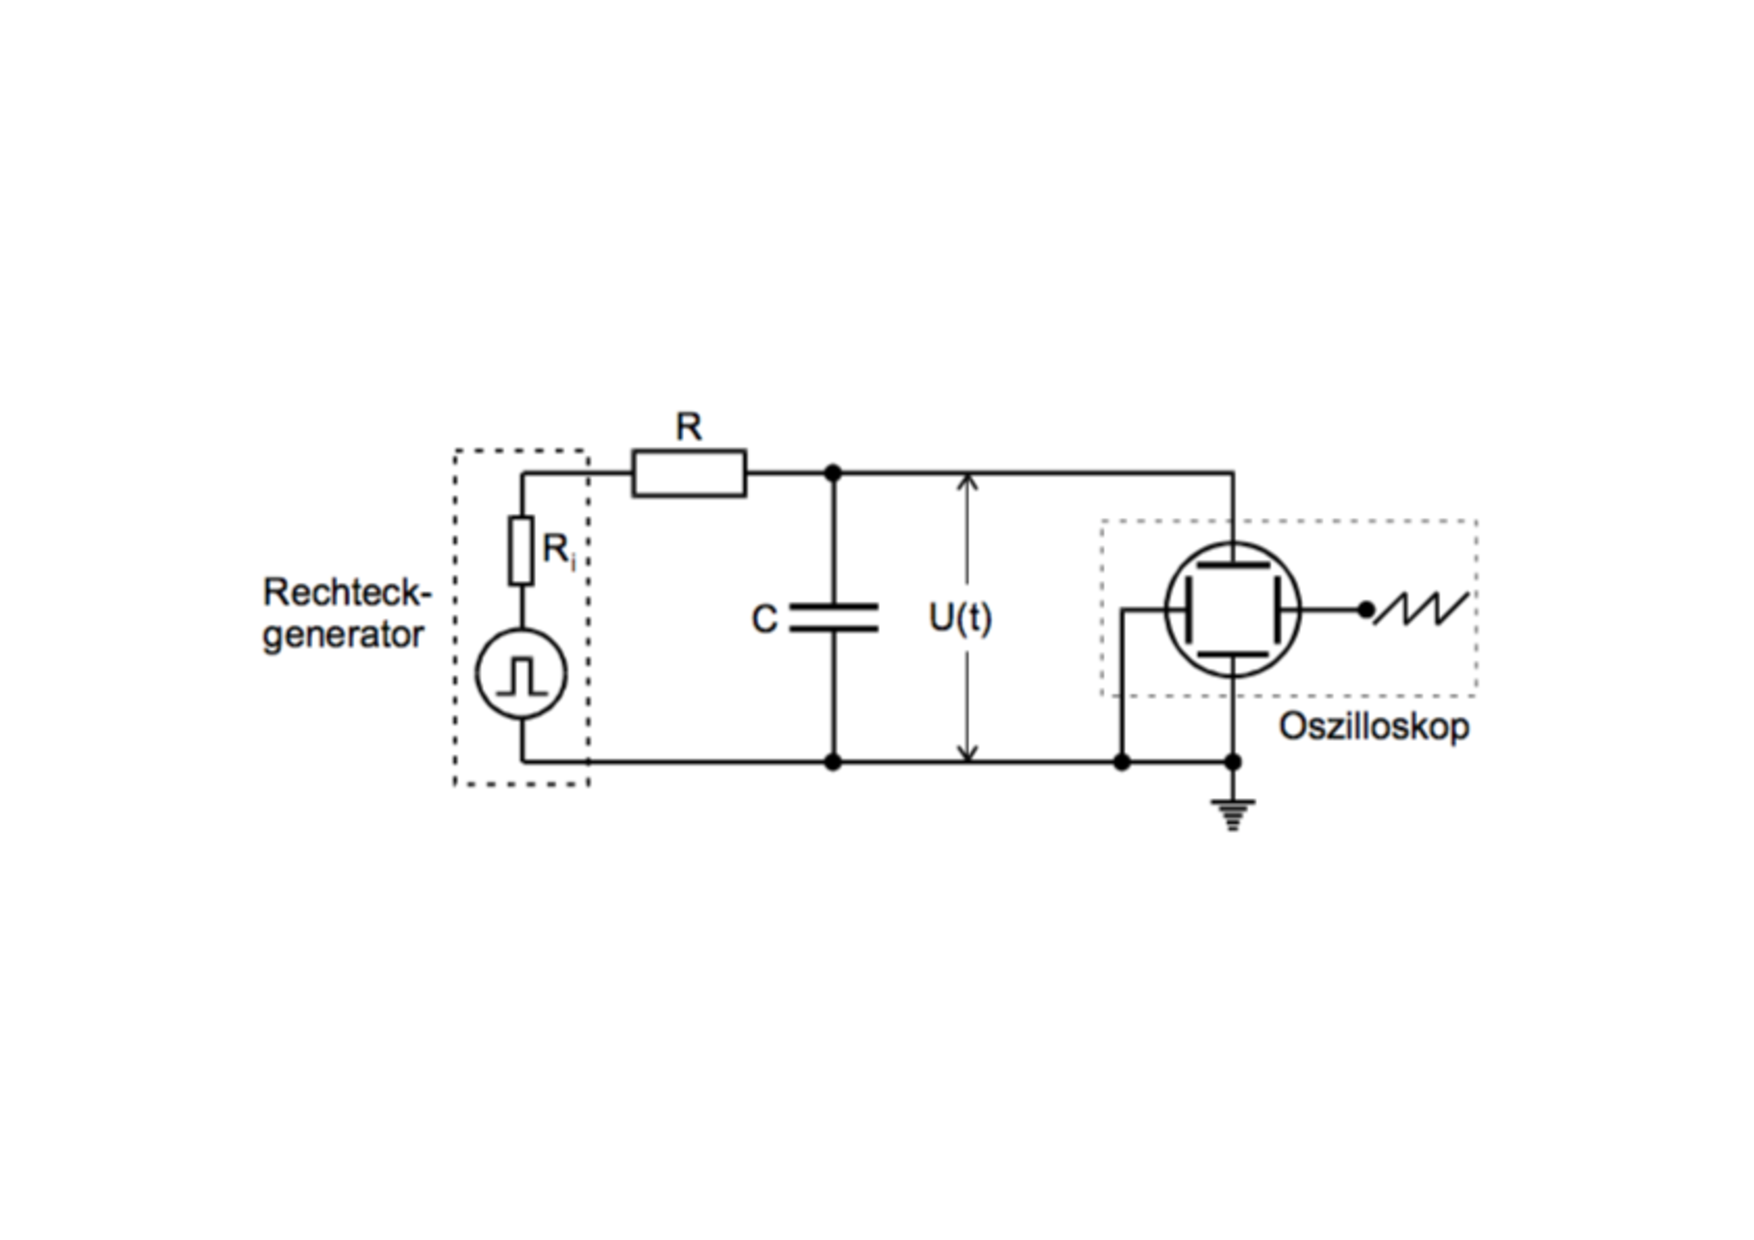
\includegraphics[width=\textwidth]{Aufbau1.pdf}
  \caption{Aufbau der Schaltung zur Bestimmung der Zeitkonstanten \cite{1}}
  \label{fig:Aufbau1}
\end{figure}

\subsection{Messreihe zur Bestimmung der Spannungsamplitude des Kondensators im RC-Kreis}
In der zweiten Messreihe wird die Spannungsamplitude der Kondensatorspannung gemessen.
Für diese Messreihe bleibt die Schaltung unverändert.
Der Spannungsgenerator wird auf Sinusspannungen $U_{0}(t)$ eingestellt.
Die Frequenz f der Spannung wird logarithmisch gesteigert.
Die jeweiligen Amplituden A werden mit dem dazugehörigen Frequenzwert notiert.
Insgesamt werden 30 Werte gemessen.

\subsection{Messreihe zur Bestimmung der Phasenverschiebung im RC-Kreis}
Die dritte Messreihe beschäftigt sich mit der Phasenverschiebung der Spannung am Kondensator und der generierten Spannung.
Die Schaltung wird zur Schaltung in Abbildung \ref{fig:Aufbau2} geändert.
Nun werden weiterhin Sinusspannungen generiert.
Auf dem Oszilloskop sind nun zwei Spannungsverläufe zu sehen: der Spannungsverlauf am Kondensator $U_{C}(t)$ und der Spannungsverlauf der generierten Spannung $U_{G}(t)$.
Wie in Abbildung \ref{fig:Phasenverschiebung} beschrieben, wird die Differenz der Nullstellen a beider Kurven und die Wellenlänge b der Kurve $U_{0}(t)$ gemessen.
Die Messung wird für 28 verschiedene Frequenzen gemacht.
Die Frequenzen werden logarithmisch gesteigert.

\begin{figure}[h!]
  \centering
  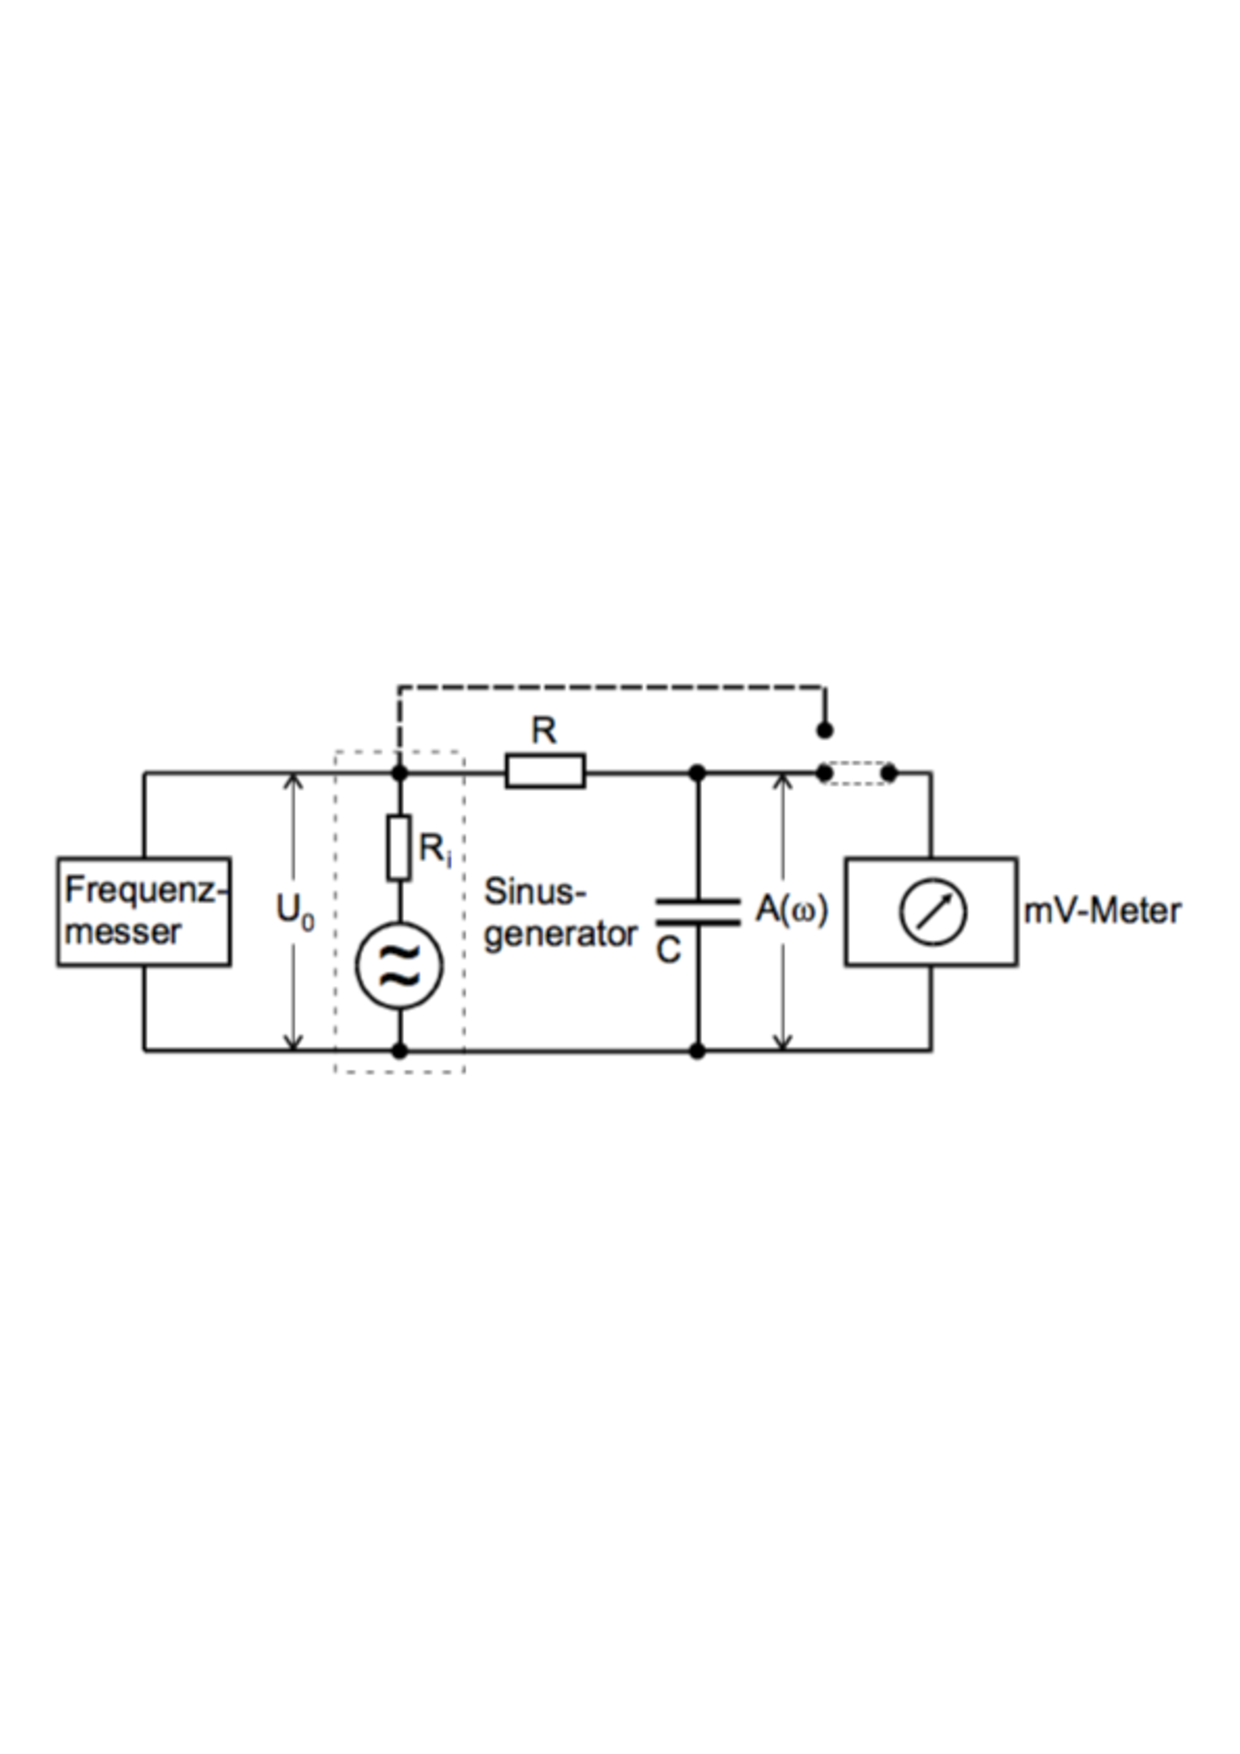
\includegraphics[width=\textwidth]{Aufbau2.pdf}
  \caption{Aufbau der Schaltung zur Bestimmung der Phasenverschiebung \cite{1}}
  \label{fig:Aufbau2}
\end{figure}

\begin{figure}[h!]
  \centering
  \includegraphics[width=\textwidth]{Phasenverschiebung.pdf}
  \caption{Skizze zur Bestimmung der Phasenverschiebung \cite{1}}
  \label{fig:Phasenverschiebung}
\end{figure}

Aus dem Abstand der Nullstellen a und der Wellenlänge b berechnet sich die Phasenverschiebung \phi über
\begin{equation}
  \phi = \frac{a}{b} \cdot 2 \pi.
\label{eqn:phasenverschiebung}
\end{equation}


\subsection{Messreihe zur Bestätigung der Integratorfunktion des RC-Kreises}
Für die vierte Messreihe wird der Aufbau abgeändert zur Schaltung in Abbildung \ref{fig:Aufbau3}.
Auf dem Oszilloskop sind nun der generierte Spannungsverlauf $U_{0}(t)$ und der integrierte Spannungsverlauf $U_{C}(t)$ zu sehen.
Zunächst wird eine Rechteckspannung am Spannungsgenerator eingestellt.
Als zweites wird eine Dreieckspannung generiert.
Die letze Einstellung ist eine Sinusspannung.
Von allen drei Bildern auf dem Oszilloskop werden Thermodrücke angefertig.

\begin{figure}[h!]
  \centering
  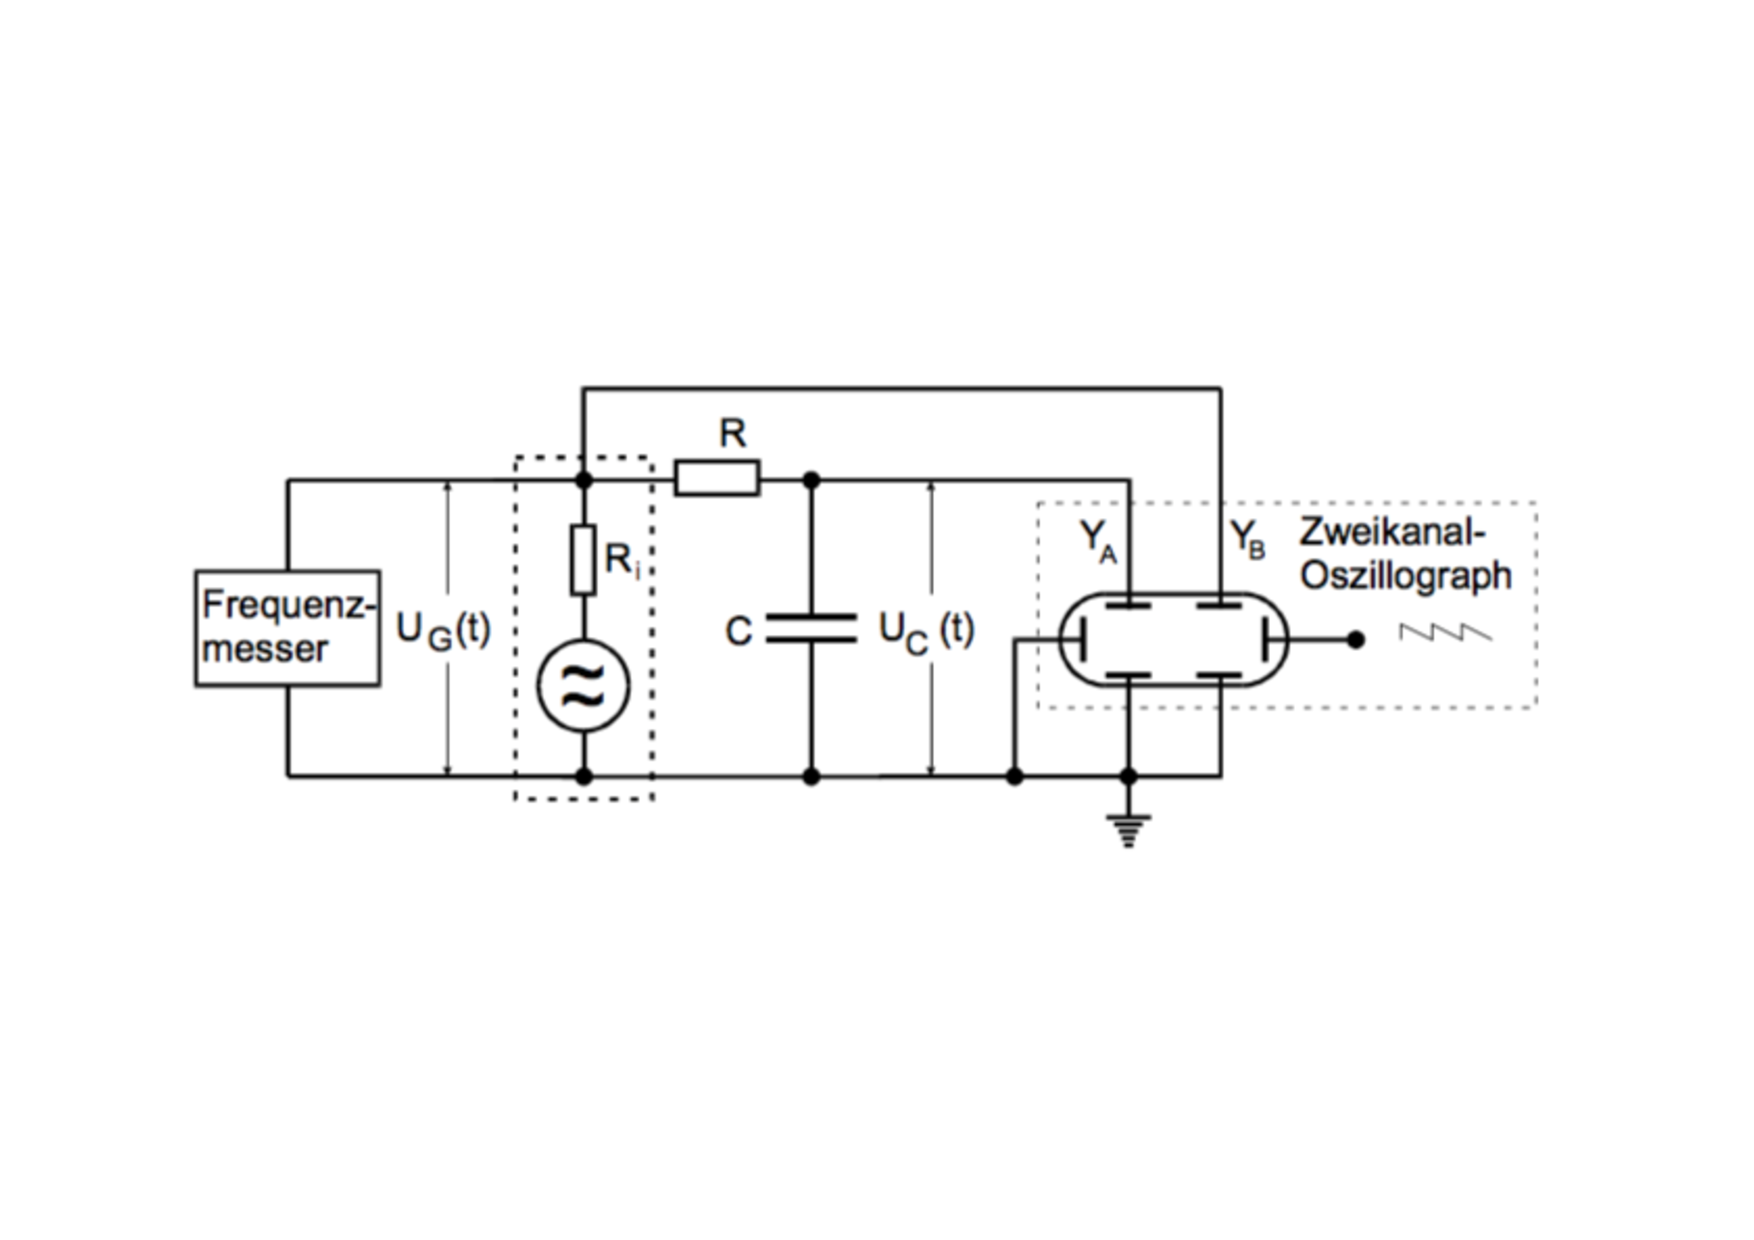
\includegraphics[width=\textwidth]{Aufbau3.pdf}
  \caption{Aufbau der dritten Schaltung \cite{1}}
  \label{fig:Aufbau3}
\end{figure}
